\documentclass[14pt]{article}
\usepackage{makeidx}
\usepackage{multirow}
\usepackage{multicol}
\usepackage[dvipsnames,svgnames,table]{xcolor}
\usepackage{graphicx}
\usepackage{epstopdf}
\usepackage{ulem}
\usepackage{hyperref}
\usepackage{amsmath}
\usepackage{amssymb}
\author{Kunal Mehta}
\title{}
\usepackage[paperwidth=595pt,paperheight=841pt,top=72pt,right=72pt,bottom=72pt,left=72pt]{geometry}

\makeatletter
	\newenvironment{indentation}[3]%
	{\par\setlength{\parindent}{#3}
	\setlength{\leftmargin}{#1}       \setlength{\rightmargin}{#2}%
	\advance\linewidth -\leftmargin       \advance\linewidth -\rightmargin%
	\advance\@totalleftmargin\leftmargin  \@setpar{{\@@par}}%
	\parshape 1\@totalleftmargin \linewidth\ignorespaces}{\par}%
\makeatother 

% new LaTeX commands


\begin{document}


\begin{center}
{\Large Project Title:}
\end{center}

\begin{center}
{\Huge \textbf{Attendance System using Face Recognition}\\}
\end{center}

\begin{center}

\end{center}
\begin{center}
{\LARGE Interns:}

\begin{enumerate}
	\item {\LARGE \textbf{Syed Mohammad Yousuff Hussain}}


{\raggedright
{\Large Email id:
\href{mailto:yousuff145@gmail.com}{yousuff145@gmail.com}}
}

{\raggedright
{\Large Contact No.: +91 97391 78327}
}


	\item {\LARGE \textbf{Kunal Jayant Mehta}}


{\raggedright
{\Large Email id:
\href{mailto:knlmht2@gmail.com}{knlmht2@gmail.com}}
}


{\raggedright
{\Large Contact No.: +91 86555 28673}
}
\end{enumerate}
\begin{center}
{\LARGE Mentors:}
\end{center}

\begin{enumerate}
	\item {\LARGE     \textbf{Yamik Mangukiya}}


{\raggedright
{\Large     Email id:
\href{mailto:yamik143@gmail.com}{yamik143@gmail.com}}
}

{\raggedright
{\Large     Contact No.: +91 90299 94989}
}


	\item {\LARGE     \textbf{Viral Bhiwandiwala}}


{\raggedright
{\LARGE     }{\Large Email id: \href{mailto:viralb101@gmail.com}{viralb101@gmail.com}}
}

{\raggedright
{\Large     Contact No.:+91 99205 39904}
}
\end{enumerate}
\end{center}
\begin{center}
{\large Duration of Internship:}
\end{center}

\begin{center}
\textbf{{\LARGE 25$^{th}$ May 2015 to 8$^{th}$ July 2015}}
\end{center}
\break
\begin{center}
{\Huge Abstract}
\end{center}

{\large This project is a part of e-Yantra Summer Internship program, 2015. The project is undertaken by Syed Mohammed Yousuff Hussain and Kunal Mehta under the guidance of Mr.Viral Bhiwandiwala and Mr.Yamik Mangukia. The end goal of this project is to build an automatic logging system using image processing for face recognition. The cameras placed at the entrance and exit of the lab will capture the image of a person entering or leaving the lab. Facial recognition on the images will be applied and the identity of the person will be extracted from the images. Sensors to determine the height of the person are placed near the entry and the exit. The height data aids the facial recognition and improves the accuracy of the system. The recognition data will be automatically logged. The system will also include a GUI application that will monitor the system and also help in viewing the logs.
	}

\break
\begin{center}
{\Huge Introduction}
\end{center}
This project involves the use of various tools of image processing to recognize faces and develop an efficient attendance recording system. Opencv library is used with Python to develop the
project on Ubuntu platform.
\begin{enumerate}
	\item \textbf{{\large About Image Processing:\\}}
In imaging science, image processing is processing of images using mathematical operations by using any form of signal processing for which the input is an image, such as a photograph or video frame; the output of image processing may be either an image or a set of characteristics or parameters related to the image. Most image-processing techniques involve treating the image as a two-dimensional signal and applying standard signal-processing techniques to it.

	\item \textbf{{\large Objectives:}}
	\begin{enumerate}
	\item The main objective is to detect and recognize face of a person entering or exiting the room thereby making attendance logging system automated.
	\item This theme can be implemented in colleges and offices to avoid wastage of time in recording attendance and avoid malpractices like proxy.
	\item We can also implement in public places like railway stations to detect and recognize criminals.\\
\end{enumerate}


	\item \textbf{{\large Tasks performed and Deadlines:}}
\end{enumerate}

{\raggedright

\vspace{3pt} \noindent
\begin{tabular}{|p{40pt}|p{311pt}|p{70pt}|}
\hline
\parbox{40pt}{\centering 
\textbf{Sr. No.}
} & \parbox{311pt}{\centering 
\textbf{Tasks}
} & \parbox{70pt}{\centering 
\textbf{Deadlines}
} \\
\hline
\parbox{40pt}{\centering 
1.
} & \parbox{311pt}{\raggedright 
Install and learn basics of python, openCV and learn Image processing modules and few exercises.
} & \parbox{70pt}{\centering 
4 days
} \\
\hline
\parbox{40pt}{\centering 
2.
} & \parbox{311pt}{\raggedright 
Face Detection from a still image and video
} & \parbox{70pt}{\centering 
4 days
} \\
\hline
\parbox{40pt}{\centering 
3.
} & \parbox{311pt}{\raggedright 
Making sample cascade “xml file”
} & \parbox{70pt}{\centering 
5 days
} \\
\hline
\parbox{40pt}{\centering 
4.
} & \parbox{311pt}{\raggedright 
Face Recognition from “image” .
} & \parbox{70pt}{\centering 
15 days
} \\
\hline
\parbox{40pt}{\centering 
5.
} & \parbox{311pt}{\raggedright 
 Face Recognition from “video input”
} & \parbox{70pt}{\centering 
5 days
} \\
\hline
\parbox{40pt}{\centering 
6.
} & \parbox{311pt}{\raggedright 
Taking a video from 2 cameras at the same time.
} & \parbox{70pt}{\centering 
3 days
} \\
\hline
\parbox{40pt}{\centering 
7.
} & \parbox{311pt}{\raggedright 
Designing algorithm for the system
} & \parbox{70pt}{\centering 
8 days
} \\
\hline
\parbox{40pt}{\centering 
	8.
} & \parbox{311pt}{\raggedright 
Making GUI for the system.
} & \parbox{70pt}{\centering 
3 days
} \\
\hline
\parbox{40pt}{\centering 
	9.
} & \parbox{311pt}{\raggedright 
Final algorithm and demo for the system
} & \parbox{70pt}{\centering 
5 days
} \\
\hline
\end{tabular}
\vspace{2pt}

}

\break

\begin{center}
{\Huge Working of the project}
\end{center}

Following shows the image of the GUI that we designed and developed for Auto logging Attendance System.
\begin{center}
	\graphicspath{ {images/} }
	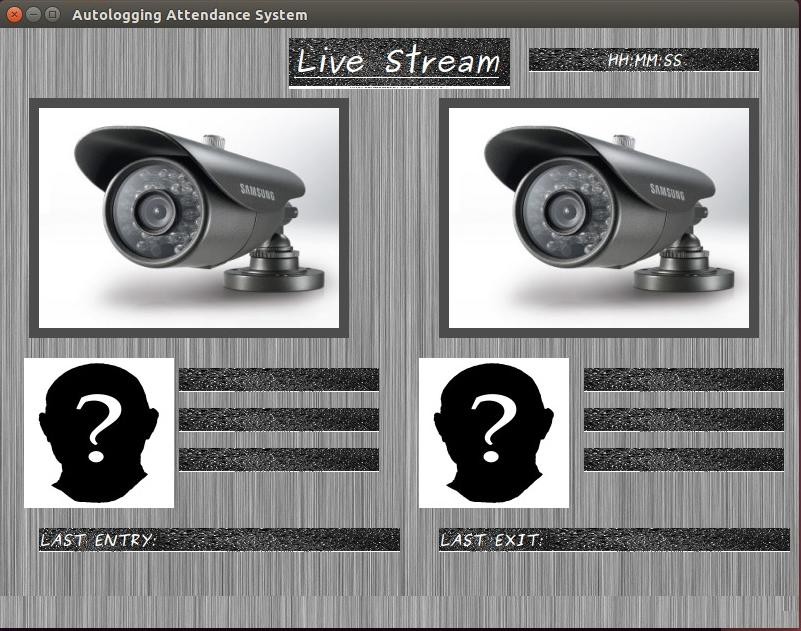
\includegraphics[width=15cm, height=8cm]{guioapp}
\end{center}
As seen in the above image, The Gui will display continuous video stream from the Entrance and Exit. The stream is basically a live stream. Initially the speed of Video in the live stream was much slower than the real time, but with the help of threading concept, speed of live stream is same as that of real time tracking. Whenever a person is detected (The detection happens when a person stands exact;y below the ultrasonic sensor used for the measurement of height) either at the entrance or the exit, his height is measured and passed to the system through serial terminal.
Depending upon the value of the height, the range in which the height fits is identified and then recognition of the person starts.
\\\\Case 1: A known Person is detected:
\\If a known person (Person from the database) is recognized either at the entrance or the exit,
his/her entry of exit time will be logged at the back end worksheet. The person is notified that
he/she is detected as soon as the green led exactly below the camera glows.
\\\\Case 2: An Unknown Person is detected:
\\If an unknown person (Person not from the database) is recognized either at the entrance or the exit, his/her entry of exit time will not be logged at the back end worksheet. In fact, his/her image will be captured and saved in a folder named 'Unknown faces' titled the date and time of his/her detection. The person is notified that he/she is detected as soon as the red led exactly below the camera glows.
\\\\Case 3: No one is detected: \\
In this case, the yellow led continues to glow.
\\\\Authority to edit the sheet:
\\Only the authorised person can edit the worksheet. Authority can be confirmed by a login Id and password.

\break

\begin{center}
{\Huge Components and its Configuration}
\end{center}

\begin{enumerate}
	\item \textbf{{\large Ultrasonic Sensor HCSR04}}


{\raggedright
This Ultrasonic sensor is interfaced with Mega ADK Arduino board for sending distance through echopin of the sensor to the pin no 8 of the arduino board.
}
	\item \textbf{{\large Arduino Mega ADK Board:}}
	\begin{enumerate}
	\item Connect Ultrasonic sensor on Arduino.
	\item Make use of USB slot for transimitting data to terminal of the Ubuntu System
	\item Connect to 7 and 8 pin no. of arduino board. 7 pin no. indicates connection to triggerpin and 8 pin no. indicates connection to echopin.
	\item Connect VCC to VCC and GND to GND ofArduino.
	\item Now turn on the system after programming it.
\end{enumerate}


	\item \textbf{{\large Cameras:}}


Two Cameras are used to capture the images or videos in real time on which the processing is done. They are connected to the USB slots of the system.
\end{enumerate}

\break

\begin{center}
{\Huge Problems faced and resolved:}
\end{center}
The project was one of the best of its kind and there were many challenges of which the most important ones are:
\begin{enumerate}
	
\item The database must be highly accurate and the expressions must be of same amenity for different
	person. Eg all the person must wink their left or right eye only. Mixture of both will not be
	considered accurate.
	\item The training of the database involves lots of mathematics and deep understanding of wide
	variety of algorithms ranging from principal component analysis through machine learning upto
	neural networks and wavelet designs. Understanding algorithms and deciding which one to use is
	a challenging task.
	\item The training of database involves training them through various layers called hidden layers with
	different weights. We trained upto 38 stages which took almost 7 to 8 hours. Still the accuracy
	was not as high as expected.
	 \item The accuracy with just image processing was not as high as expected and the results were with
	some error. However this error was reduced greatly using height integration. It can be further
	reduced by integrating weight.
	 \item Designing GUI from a wide range of available Python libraries was challenging since none of
	the library supported direct video streaming. So we started saving images with 30fps and then
	reading them into the GUI. Thus using persistence of vision concept to make those images being
	viewed as a continuous video.

\end{enumerate}
\break

\begin{center}
{\Huge Future Scope}
\end{center}

\begin{enumerate}
	\item  We can add the data of newly joined employee in the database at the run time.
	 \item An android app can be created so as to ensure all the employees to check whether their
	attendance is marked or not.
	\item Gui can be made more lively by adding features like background optimizations.
	 \item We can even add an LCD display below the camera were a person can see his/her name or ID
	when detected and recognized.
	\item  We can even make a sophisticated system where the door of the room automatically opens or
	closes on detection of the person, making it smart room or smart office.
\end{enumerate}

\break

\newpage
\begin{center}
{\Huge References}
\end{center}

\begin{itemize}
	\item Firebird V hardware and software manuals.
	\item Neurosky Mindwave Headset datasheets.
	\item JY-MCU and HC-05 Bluetooth module datasheets.
	\item https://en.wikipedia.org/wiki/Electroencephalograph
	\item http://neurosky.com/biosensors/eeg-sensor/biosensors/
	\item https://learn.sparkfun.com/tutorials/hackers-in-residence---hacking-mindwave-mobile
	\item https://www.pantechsolutions.net/mind-attention-control-led-using-arduino
	\item https://www.pantechsolutions.net/mind-meditation-control-led-using-arduino
	\item https://www.pantechsolutions.net/eye-blink-control-led-using-arduino
\end{itemize}
\hspace{15pt}

\newpage
\begin{center}
	{\Huge Softwares used on Ubuntu:}
\end{center}
\begin{itemize}
	\item Python and its libraries 
	\begin{itemize}
		\item MatPlotlib
		\item PyQt4
		\item NumPy
		\item CV2
		\item xlrd, xlwt, xlutils
		\item serial
	\end{itemize}
	\item OpenCV
	\item Arduino IDE
	\item QtDesigner for Designing GUI
\end{itemize}

\end{document}